%%
%% Concepts
%%
%% This file should be edited by user
%%

\chapter{Concepts} \label{chapter:concepts}

Usually, this chapter is necessary in order to give an overview on
the \emph{terms} and \emph{concepts} that are required to understand
your work.

\section{Writing Style}

Usually you should not use the first person singular (\emph{I}) in
your text, write \emph{we} instead. As a general recommendation, use
the first person sparsely, sometimes it can be replaced by a phrase
like \emph{This work presents...}.

The indefinite article \textbf{a} is used as \textbf{an} before a
vowel sound - for example \textbf{an} apple, \textbf{an} hour,
\textbf{an} unusual thing, \textbf{an} FPGA (becourse the acronym is
pronouned Ef-Pee-Gee-A), \textbf{an} HIL. Before a consonant sound
represented by a vowel letter \textbf{a} is usual -- for example
\textbf{a} one, \textbf{a} unique thing, \textbf{a} historic
chance\footnote{According to Merriam Webster, both \textbf{a} and
\textbf{an} can be used in writing before unstressed or weakly
stressed syllables with initial h, thus you could also write
\textbf{an} historic chance.}.

\section{Acronyms}

Explain acronyms at their first occurrence in the text. In order to
achieve this consistently, we recommend to use the \texttt{acronym}
package.

A new acronym is then declared by writing
\verb+\newacro{acronym}{expanded name}+. Use the macro
\verb+\ac{acronym}+ as a placeholder for the acronym in the text.

See file \texttt{acronym.tex} for further examples and explanations.

\newacro{GPL}{Gnu Public License}

\section{Figures}

A Figure should always be referenced in the text, as it is the case
with Figure~\ref{fig:example}.

\begin{figure}[h]
 \centerline{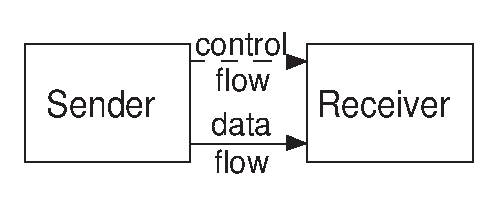
\includegraphics[width=.5\columnwidth]{pics/example}}
  \caption{Example figure}
  \label{fig:example}
\end{figure}

This template can be compiled with the \texttt{latex} command or the
\texttt{pdflatex} command. While \texttt{latex} creates an
intermediate file format (.dvi) that can be further processed into a
\texttt{.ps} or \texttt{.pdf} file, the \texttt{pdflatex} command
directly creates a \texttt{.pdf} file.

Note that with \texttt{latex} the \verb+\includegraphics+ accepts
only .eps files, while with \texttt{pdflatex} accepts \texttt{.pdf},
\texttt{.png}, or \texttt{.jpg}. Luckily, the file extension can be
omitted in order that \verb+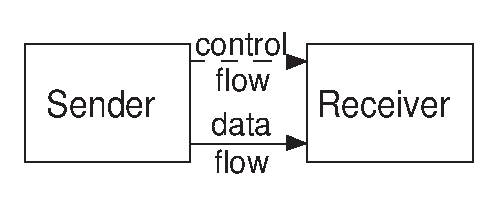
\includegraphics{pics/example}+ will
look for file with name \texttt{example.eps} in \texttt{latex} mode
and for a file with name \texttt{example.pdf}, \texttt{example.png},
or \texttt{example.jpg} in \texttt{pdflatex} mode. If you already
have an \texttt{.eps} file, you may create a respective
\texttt{.pdf} file with the commandline conversion tool
\texttt{epstopdf}.

\section{Citations and References}

Whenever you refer to previously published work, you should set a
reference to acknowledge the work you build upon. For example this
is a reference to two bachelor's theses~\cite{kraut:2003,
weirich:2005}. If you literally cite a part of someone else's work,
mark the respective sentence by quotes and italic letters and add
the page number, where is text can be found:

\dqit{An intelligent or {\em smart} transducer is the integration of
an analog or digital sensor or actuator element, a processing unit,
and a communication interface. In case of a sensor, the smart
transducer transforms the raw sensor signal to a standardized
digital representation, checks and calibrates the signal, and
transmits this digital signal to its users via a standardized
communication protocol.}\cite[p.\,175]{elmenreich:2005}

\section{Spellchecking}

Do not use your advisor as your spell checker. Instead, run an
electronic spell checker over your document before submitting the
document to your advisor.

\section{References with Bibtex}

Bibtex is an additional program to {\LaTeX} that creates a list of
your cited references in a chapter named {\em Bibliography}. In
order to use Bibtex, you must maintain a database of all references
in so-called \emph{bibfiles} (file extension \texttt{.bib}).

The \emph{bibfiles} contain entries of several types, the most
needed types are \texttt{book}, \texttt{inproceedings},
\texttt{article}, \texttt{techreport}, \texttt{mastersthesis}, and
\texttt{phdthesis}. In the following we list the templates for these
types, whereas each asterisk (*) should be replaced by the
respective data, if this is not available, the element should be
left out. The case of the element names does not matter to Bibtex,
however in the examples we have used UPPERCASE for the obligatory
fields and lowercase for the optional fields. To see some complete
examples, have a look into the file \texttt{bibfile.bib}. For more
information, read~\cite{patashnik:1988}.

\subsection{Some BibteX Examples}

\footnotesize
\begin{verbatim}
@BOOK{*,
  AUTHOR =       {*},
  editor =       {*},
  TITLE =        {*},
  PUBLISHER =    {*},
  YEAR =         {*},
  volume =       {*},
  number =       {*},
  series =       {*},
  address =      {*},
  edition =      {*},
  month =        {*},
  note =         {*}
}

@INPROCEEDINGS{*,
  AUTHOR =       {*},
  TITLE =        {*},
  BOOKTITLE =    {*},
  YEAR =         {*},
  editor =       {*},
  volume =       {*},
  number =       {*},
  series =       {*},
  pages =        {*},
  address =      {*},
  month =        {*},
  organization = {*},
  publisher =    {*},
  note =         {*}
}

@ARTICLE{*,
  AUTHOR =       {*},
  TITLE =        {*},
  JOURNAL =      {*},
  YEAR =         {*},
  volume =       {*},
  number =       {*},
  pages =        {*},
  month =        {*},
  note =         {*}
}

@TECHREPORT{*,
  AUTHOR =       {*},
  TITLE =        {*},
  INSTITUTION =  {*},
  YEAR =         {*},
  type =         {*},
  number =       {*},
  address =      {*},
  month =        {*},
  note =         {*}
}

@MASTERSTHESIS{*,
  AUTHOR =       {*},
  TITLE =        {*},
  SCHOOL =       {*},
  YEAR =         {*},
  type =         {*},
  address =      {*},
  month =        {*},
  note =         {*}
}

@PHDTHESIS{*,
  AUTHOR =       {*},
  TITLE =        {*},
  SCHOOL =       {*},
  YEAR =         {*},
  type =         {*},
  address =      {*},
  month =        {*},
  note =         {*},
  abstract =     {*},
  keywords =     {*},
  source =       {*},
} \end{verbatim}




%%
%% = eof =====================================================================
%%
